\documentclass[aspectratio=169]{beamer}
\usepackage{fontspec}

% Tipografías de la Identidad Visual
\setmainfont{Inter}
\setsansfont{Inter}
\setmonofont{JetBrains Mono}
\newfontfamily\titlefont{Montserrat}[BoldFont={Montserrat Bold}]

% Colores de la Identidad Visual
\definecolor{AzulMarino}{HTML}{1A365D}
\definecolor{GrisPizarra}{HTML}{4A5568}
\definecolor{BlancoNieve}{HTML}{F7FAFC}
\definecolor{VerdeAzulado}{HTML}{319795}

% Aplicación de colores a Beamer
\setbeamercolor{palette primary}{bg=AzulMarino, fg=BlancoNieve}
\setbeamercolor{palette secondary}{bg=VerdeAzulado, fg=BlancoNieve}
\setbeamercolor{palette tertiary}{bg=GrisPizarra, fg=BlancoNieve}
\setbeamercolor{structure}{fg=AzulMarino}
\setbeamercolor{background canvas}{bg=BlancoNieve}
\setbeamercolor{normal text}{fg=GrisPizarra}

\setbeamerfont{title}{family=\titlefont, series=\bfseries, size=\Huge}
\setbeamerfont{frametitle}{family=\titlefont, series=\bfseries, size=\LARGE}

\usepackage[utf8]{inputenc}
\usepackage{graphicx}
\usepackage{amsmath}

\title{Preprocesamiento y Limpieza de Datos}
\subtitle{Diagnóstico, Nulos, Codificación y Escalamiento (Teoría)}
\author{Clase Teórica - Semana 2}
\date{}

\begin{document}

\begin{frame}
    \titlepage
\end{frame}

\begin{frame}{El Rompecabezas Dañado (Valores Nulos)}
    ¿Qué hacer cuando faltan datos (\texttt{NaN})?
    \begin{itemize}
        \item \textbf{\textcolor{AzulMarino}{Tirar a la Basura (\texttt{dropna}):}} Eliminamos el registro. Fácil, pero perdemos información.
        \item \textbf{La Media Aritmética (\texttt{mean}):} Promediamos los datos. Peligroso si hay valores extremadamente altos que sesguen.
        \item \textbf{\textcolor{VerdeAzulado}{La Mediana (\texttt{median}):}} El valor seguro del medio. Inmune a las anomalías extremas.
    \end{itemize}
\end{frame}

\begin{frame}{Cajas de Luz (One-Hot Encoding)}
    Los algoritmos no entienden palabras, solo números. Si tenemos las clases de malware: \textit{Trojan}, \textit{Ransomware}, \textit{Phishing}.
    
    \vspace{0.3cm}
    \textbf{Peligro (Label Encoding):} \\
    Trojan = 0, Ransomware = 1, Phishing = 2. \\
    ¡El algoritmo pensará que Phishing (2) "vale" más que Trojan (0)!
    
    \vspace{0.3cm}
    \textbf{\textcolor{VerdeAzulado}{Solución (One-Hot):}} \\
    Creamos 3 columnas binarias. Trojan = \texttt{[1, 0, 0]}. Phishing = \texttt{[0, 0, 1]}. \textbf{Equidad matemática.}
\end{frame}

\begin{frame}{El Álbum de Stickers (Escalamiento Dimensional)}
    Si tienes Sueldo (0 a \$1M) y Edad (0 a 100), el algoritmo que calcule "distancias" ignorará la Edad.
    
    \begin{alertblock}{Soluciones Matemáticas}
    \begin{itemize}
        \item \textbf{MinMaxScaler:} Acota matemáticamente los datos a un rango estricto \([0, 1]\). Destruido fácilmente si un Outlier gigante estira demasiado el marco.
        \item \textbf{\textcolor{VerdeAzulado}{StandardScaler:}} Ajusta los datos para que tengan un promedio de 0 y varianza de 1. Se basa en cuánto te desvías del grupo.
    \end{itemize}
    \end{alertblock}
\end{frame}

\begin{frame}{Detección de Outliers (IQR)}
    \begin{center}
        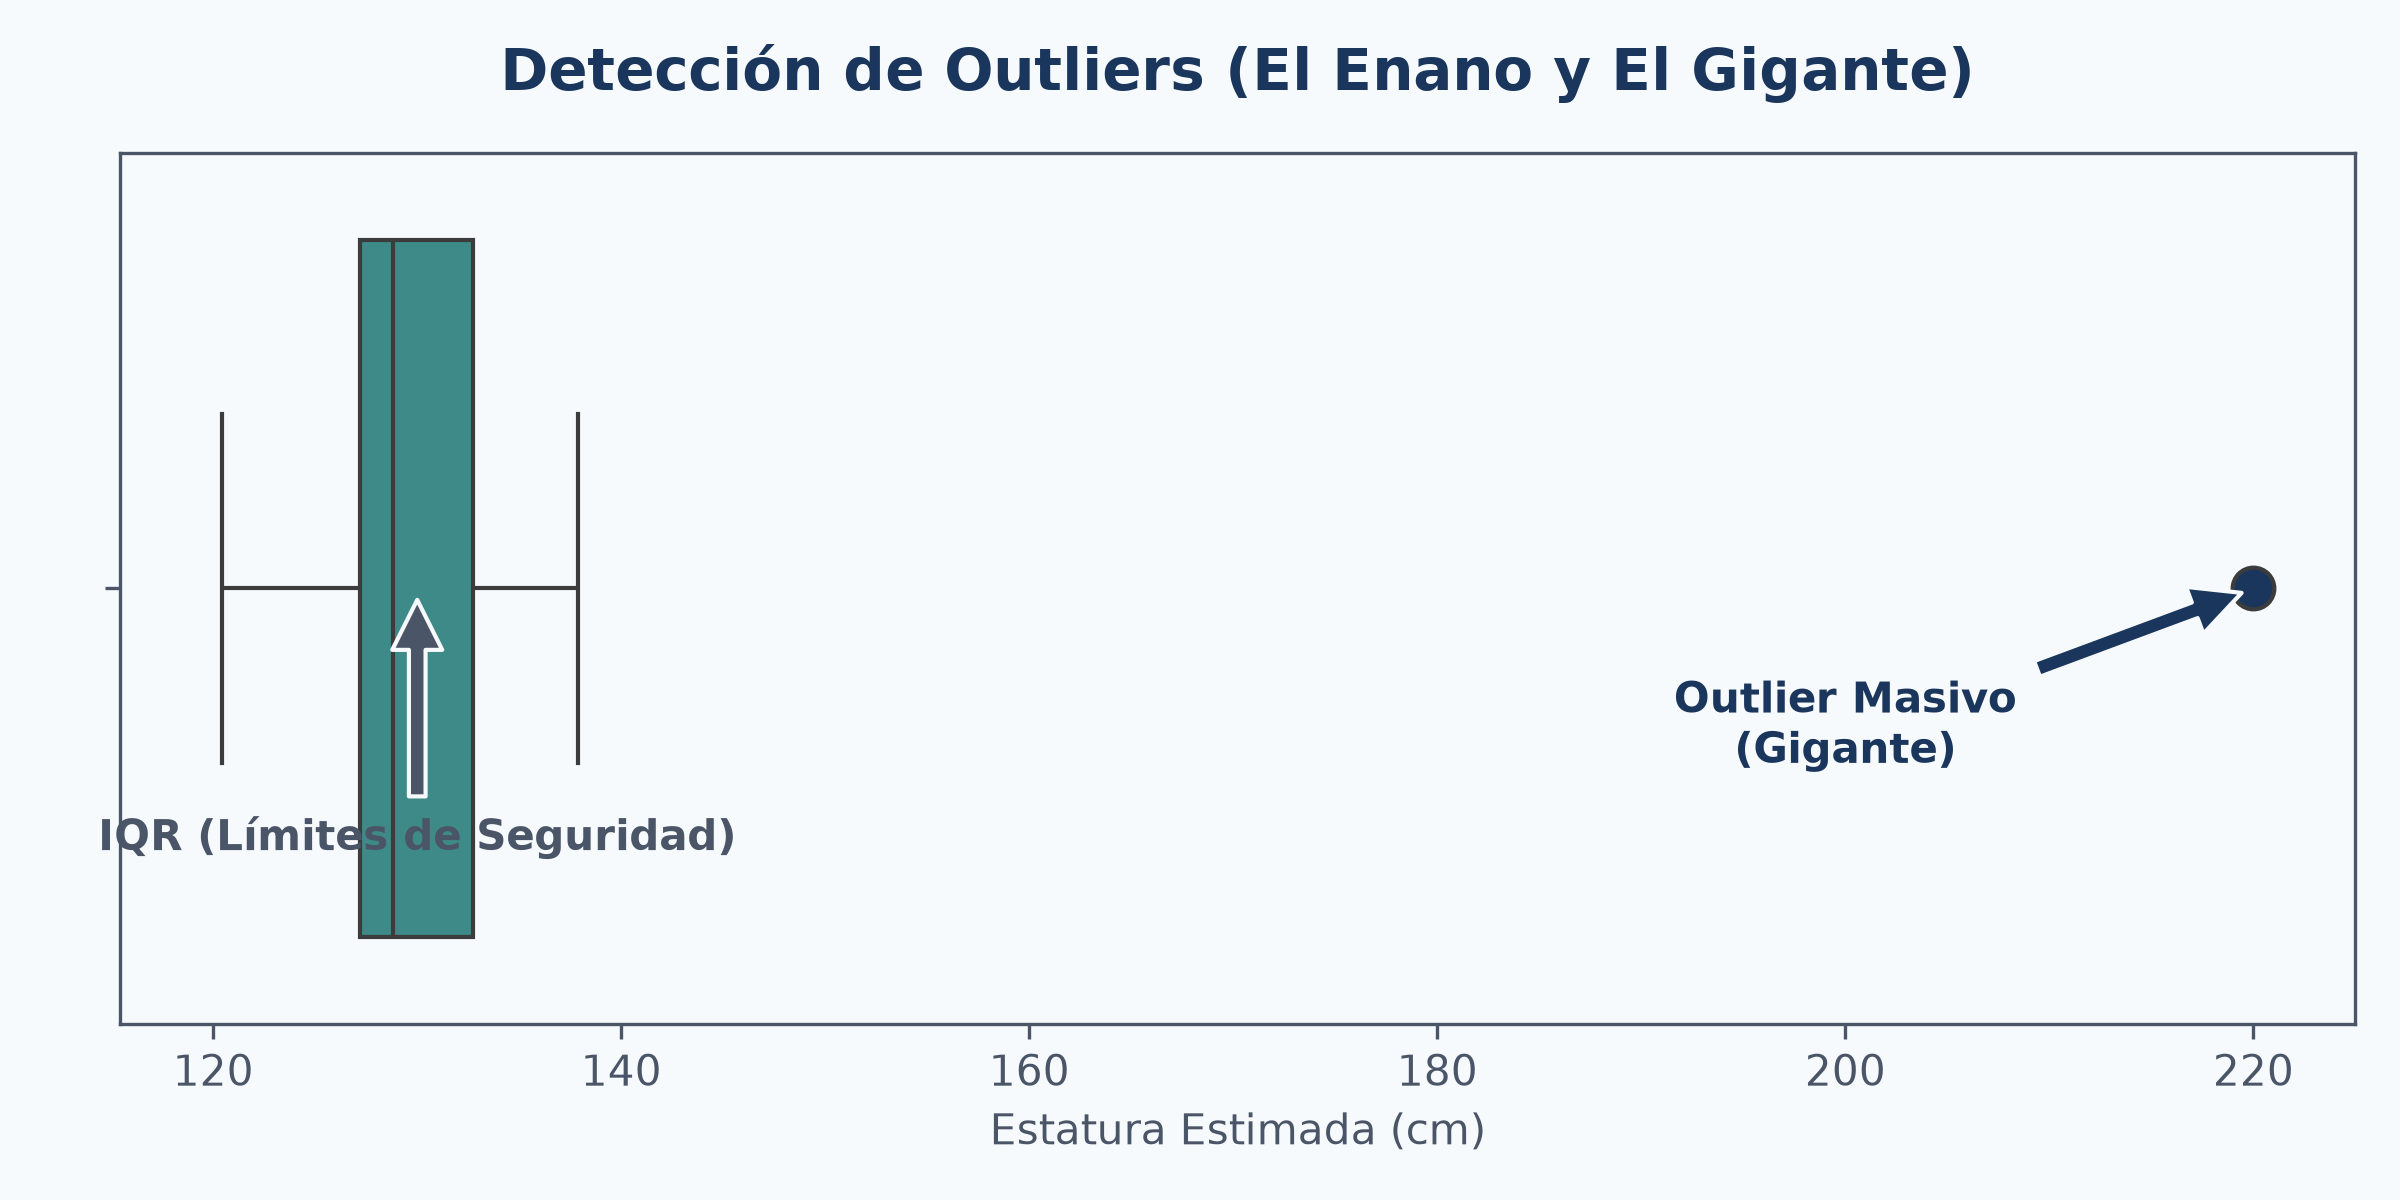
\includegraphics[width=0.7\textwidth]{outlier_concept.png}
    \end{center}
    Una frontera estadística nos ayuda a identificar si una transmisión de red de 1TB es un ataque (outlier) o comportamiento normal.
\end{frame}

\end{document}
